% TikZ diagram of the Two-Step and One-Step cascades (Section "Architecture"); no extra packages.
\usetikzlibrary{arrows.meta}
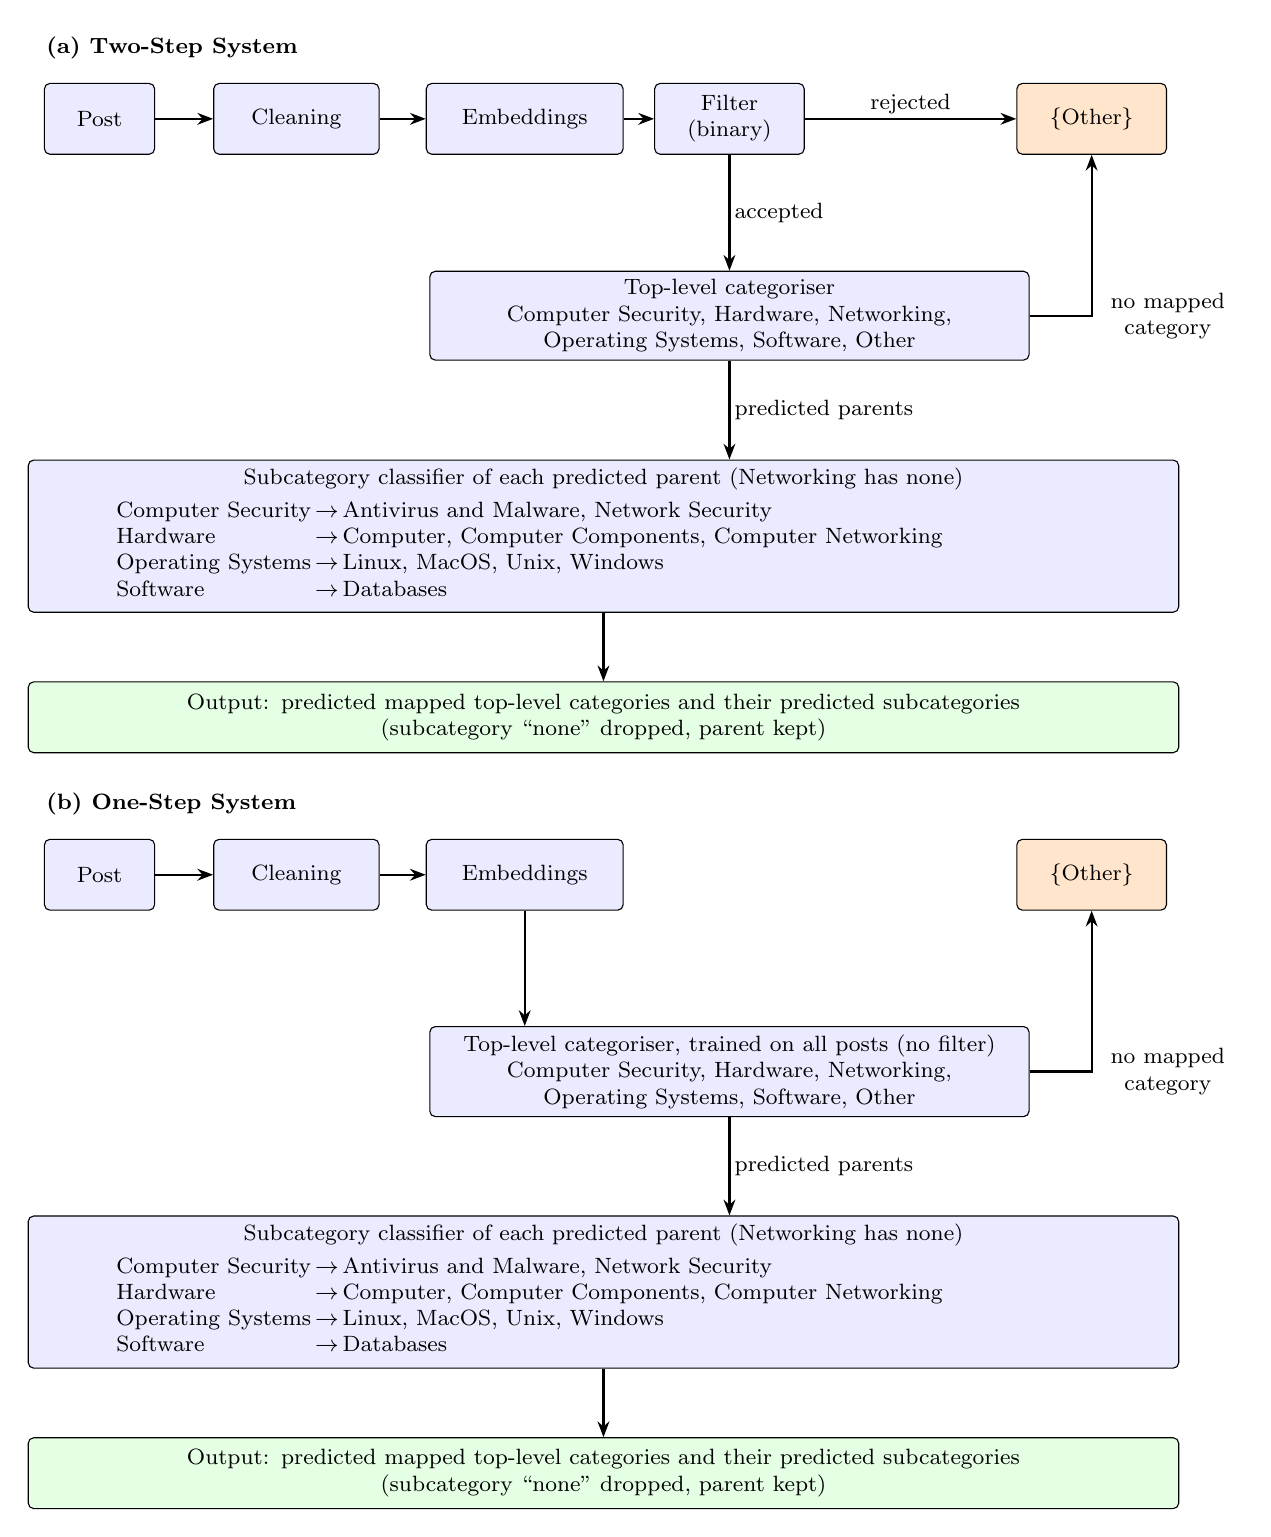
\begin{tikzpicture}[
    font=\footnotesize,
    >={Stealth[length=2mm]},
    box/.style={draw, rounded corners=2pt, fill=blue!8, align=center, minimum height=0.9cm, inner sep=3pt},
    other/.style={draw, rounded corners=2pt, fill=orange!20, align=center, minimum height=0.9cm, inner sep=3pt},
    result/.style={draw, rounded corners=2pt, fill=green!10, align=center, minimum height=0.9cm, inner sep=3pt},
    flow/.style={->, thick},
    lab/.style={font=\footnotesize, inner sep=1.5pt, fill=white}
]
\node[anchor=west, font=\footnotesize\bfseries] at (0,0.9) {(a) Two-Step System};
\node[box, minimum width=1.4cm] (a1) at (0.8,0) {Post};
\node[box, minimum width=2.1cm] (a2) at (3.3,0) {Cleaning};
\node[box, minimum width=2.5cm] (a3) at (6.2,0) {Embeddings};
\node[other, minimum width=1.9cm] (ao) at (13.4,0) {\{Other\}};
\draw[flow] (a1) -- (a2);
\draw[flow] (a2) -- (a3);
\node[box, minimum width=1.9cm] (af) at (8.8,0) {Filter\\(binary)};
\draw[flow] (a3) -- (af);
\draw[flow] (af) -- node[lab, above] {rejected} (ao);
\node[box, text width=7.4cm] (at) at (8.8,-2.5) {Top-level categoriser\\Computer Security, Hardware, Networking,\\Operating Systems, Software, Other};
\draw[flow] (at.east) -| node[lab, pos=0.5, right, text width=1.8cm, align=center, fill=none] {no mapped category} (ao.south);
\draw[flow] (af) -- node[lab, right] {accepted} (at);
\node[box, text width=14.4cm] (as) at (7.2,-5.3) {Subcategory classifier of each predicted parent (Networking has none)\\[2pt]
    \begin{tabular}{@{}l@{\,$\rightarrow$\,}p{9.5cm}@{}}
    Computer Security & Antivirus and Malware, Network Security\\
    Hardware & Computer, Computer Components, Computer Networking\\
    Operating Systems & Linux, MacOS, Unix, Windows\\
    Software & Databases
    \end{tabular}};
\node[result, text width=14.4cm] (aout) at (7.2,-7.6) {Output: predicted mapped top-level categories and their predicted subcategories\\(subcategory ``none'' dropped, parent kept)};
\draw[flow] (at.south) -- node[lab, right] {predicted parents} (at.south |- as.north);
\draw[flow] (as) -- (aout);
\begin{scope}[yshift=-9.6cm]
\node[anchor=west, font=\footnotesize\bfseries] at (0,0.9) {(b) One-Step System};
\node[box, minimum width=1.4cm] (b1) at (0.8,0) {Post};
\node[box, minimum width=2.1cm] (b2) at (3.3,0) {Cleaning};
\node[box, minimum width=2.5cm] (b3) at (6.2,0) {Embeddings};
\node[other, minimum width=1.9cm] (bo) at (13.4,0) {\{Other\}};
\draw[flow] (b1) -- (b2);
\draw[flow] (b2) -- (b3);
\node[box, text width=7.4cm] (bt) at (8.8,-2.5) {Top-level categoriser, trained on all posts (no filter)\\Computer Security, Hardware, Networking,\\Operating Systems, Software, Other};
\draw[flow] (bt.east) -| node[lab, pos=0.5, right, text width=1.8cm, align=center, fill=none] {no mapped category} (bo.south);
\draw[flow] (b3.south) -- (b3.south |- bt.north);
\node[box, text width=14.4cm] (bs) at (7.2,-5.3) {Subcategory classifier of each predicted parent (Networking has none)\\[2pt]
    \begin{tabular}{@{}l@{\,$\rightarrow$\,}p{9.5cm}@{}}
    Computer Security & Antivirus and Malware, Network Security\\
    Hardware & Computer, Computer Components, Computer Networking\\
    Operating Systems & Linux, MacOS, Unix, Windows\\
    Software & Databases
    \end{tabular}};
\node[result, text width=14.4cm] (bout) at (7.2,-7.6) {Output: predicted mapped top-level categories and their predicted subcategories\\(subcategory ``none'' dropped, parent kept)};
\draw[flow] (bt.south) -- node[lab, right] {predicted parents} (bt.south |- bs.north);
\draw[flow] (bs) -- (bout);
\end{scope}
\end{tikzpicture}
